\chapter{T-536 program}
\label{chap:program}

\section{Experimental setup}

An overview of the experiment setup is shown in figure~\ref{fig:overview}.
%
The calorimeter system is located inside the tunnel,
the laser system is located just outside of it and 
the DAQ backend and analysis machines are located in the control room
several floors above the tunnel.
%
Detailed description of each sub-system is given in the subsequent sections. 
%
\begin{figure}[htbp]
\centering
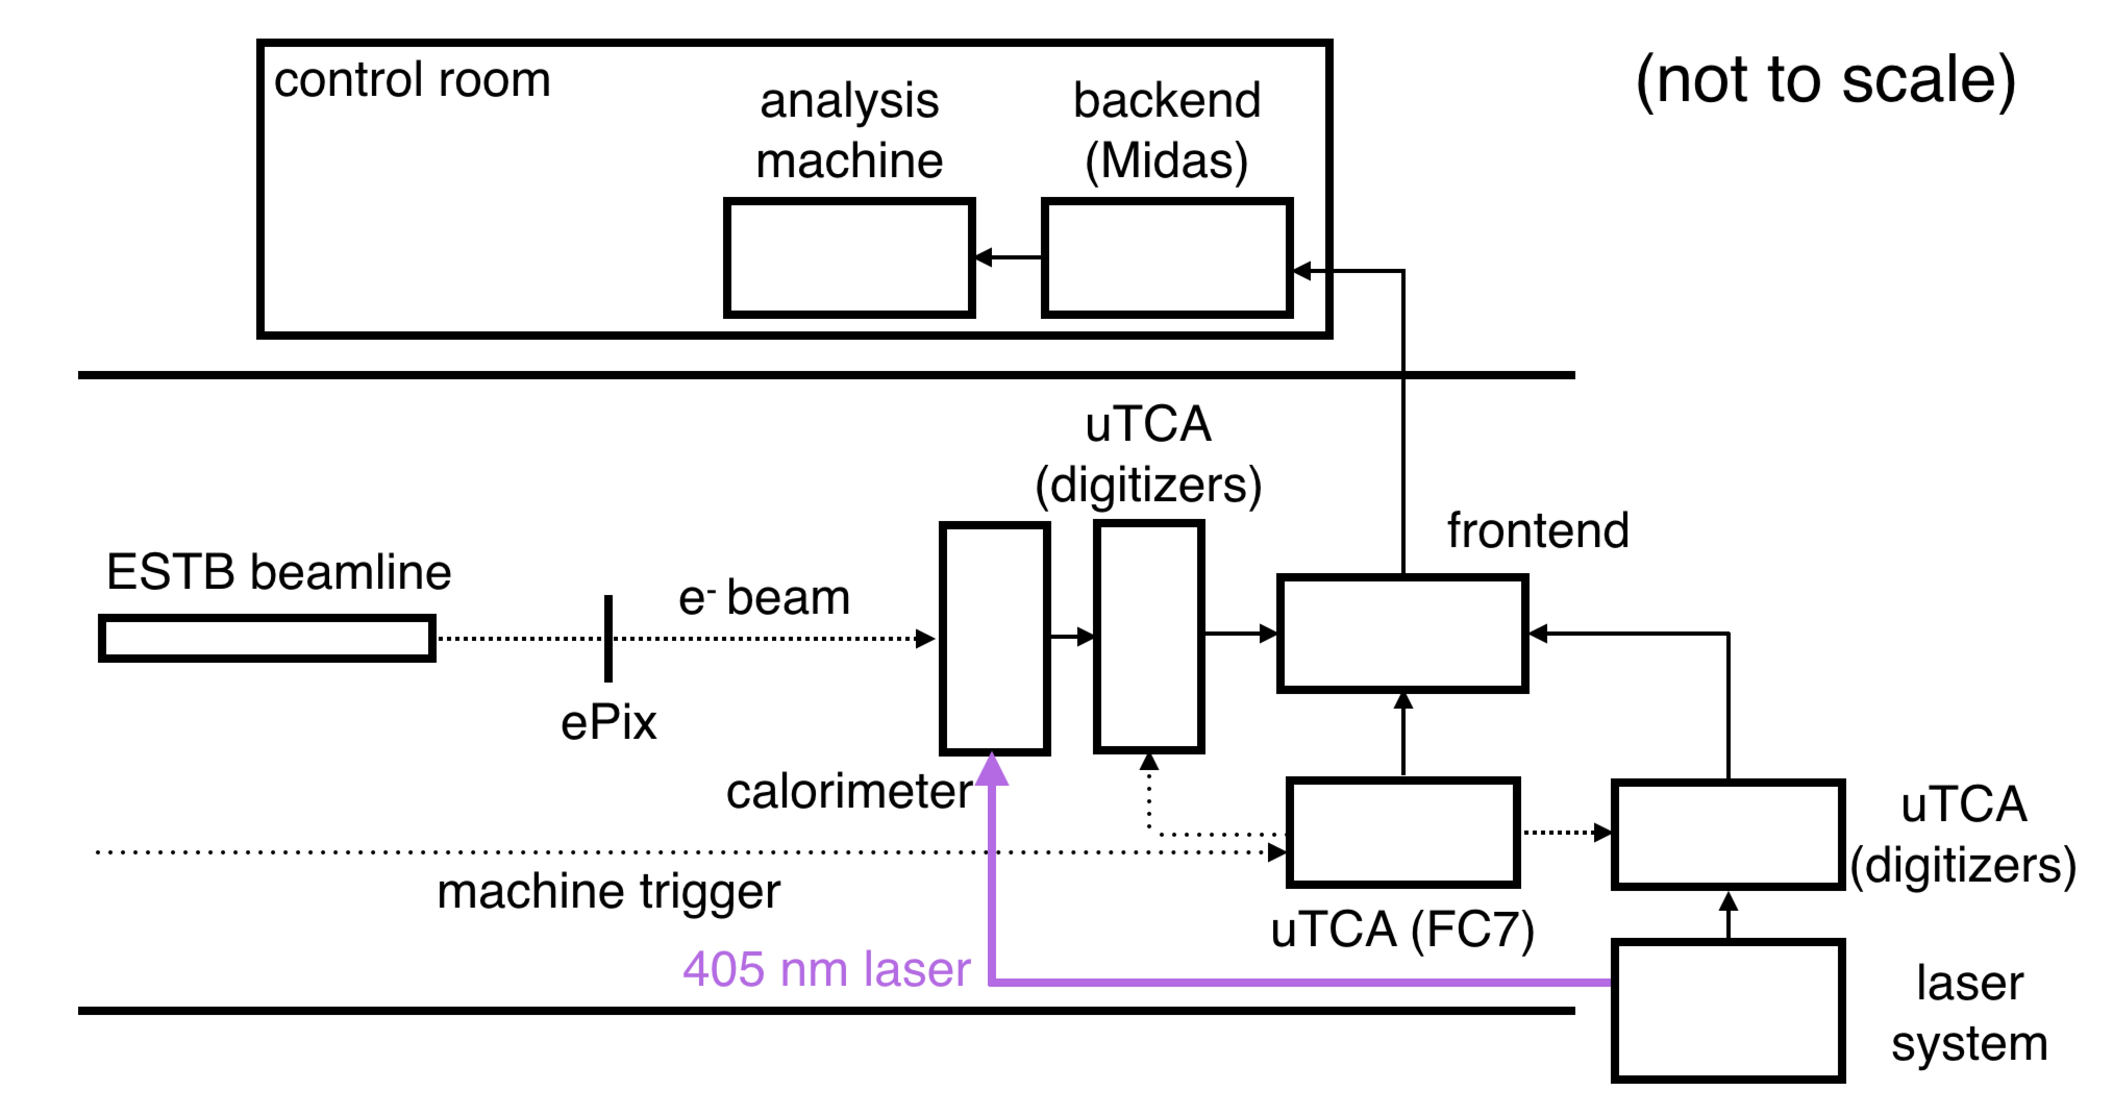
\includegraphics[width=.85\textwidth]{pics/SLACoverview}
\caption{Overview of the experimental setup at SLAC. 
Electron beam from the ESTB beamline is moving from
the left to right before hitting the calorimeter.
The SiPM pulses resulting from the EM shower are digitized and
then processed by the frontend and backend machines to be ready for data analysis.
}\label{fig:overview}
\end{figure}

\section{Mapping of the Calorimeter and the Waveform digitizer WFD5}

For data analyses related to the timing resolution extraction from timing difference, it is very important to know if both channels are coming from the same or different WFD5. In Fig.~\ref{fig:calowfd5map},
the calorimeter crystal number is given at the right bottom corner and the WFD5's AMC slot number in a $\mu$TCA crate is given in R$N$ where $N$ is the slot number.

\begin{figure}[htbp]
\centering
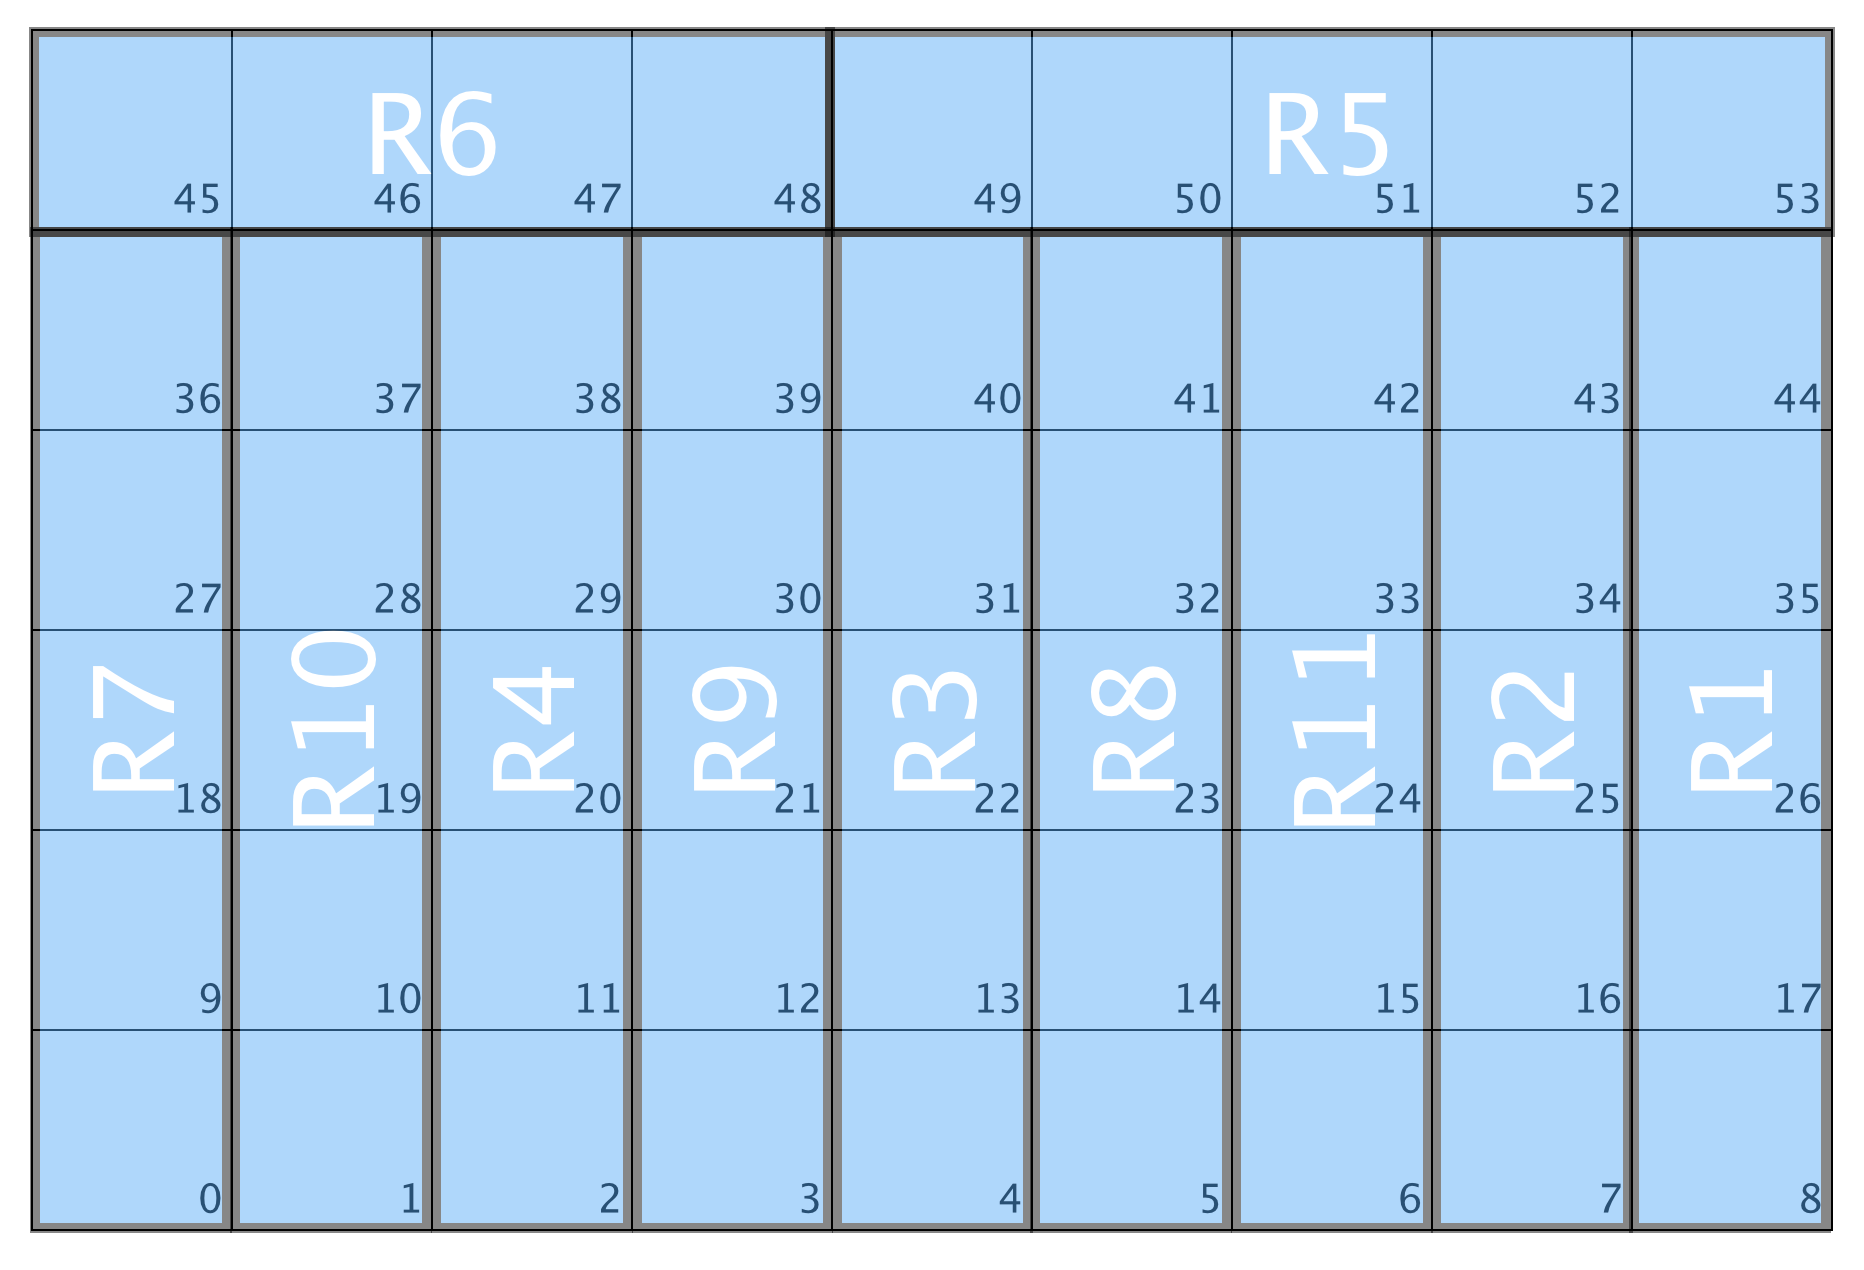
\includegraphics[width=.7\textwidth]{pics/CaloWFD5Map}
\caption{\label{fig:calowfd5map}A mapping between calorimeter crystal number and the WFD5 AMC slot number.}
\end{figure}

\section{Event topology}

Understanding the SLAC event topology is a crucial step in the data analysis.
At the beginning of each fill, a sync laser pulsed is fired for timing alignment purpose. This pulse shows up at around 1~$\mu$s ($\approx$ 800 c.t.) in the digitizer.
Then the electron beam will arrive at about 3~$\mu$s ($\approx$ 2400 c.t.).
For the rest of the time until 700 $\mu$s, laser pulses for laser calibration and SiPM gain monitoring purpose will be firing at either 10 kHz or 100 kHz depending on the runs.
A typical recorded waveform is shown in Fig.~\ref{fig:eventtopology}.

\begin{figure}[htbp]
\centering
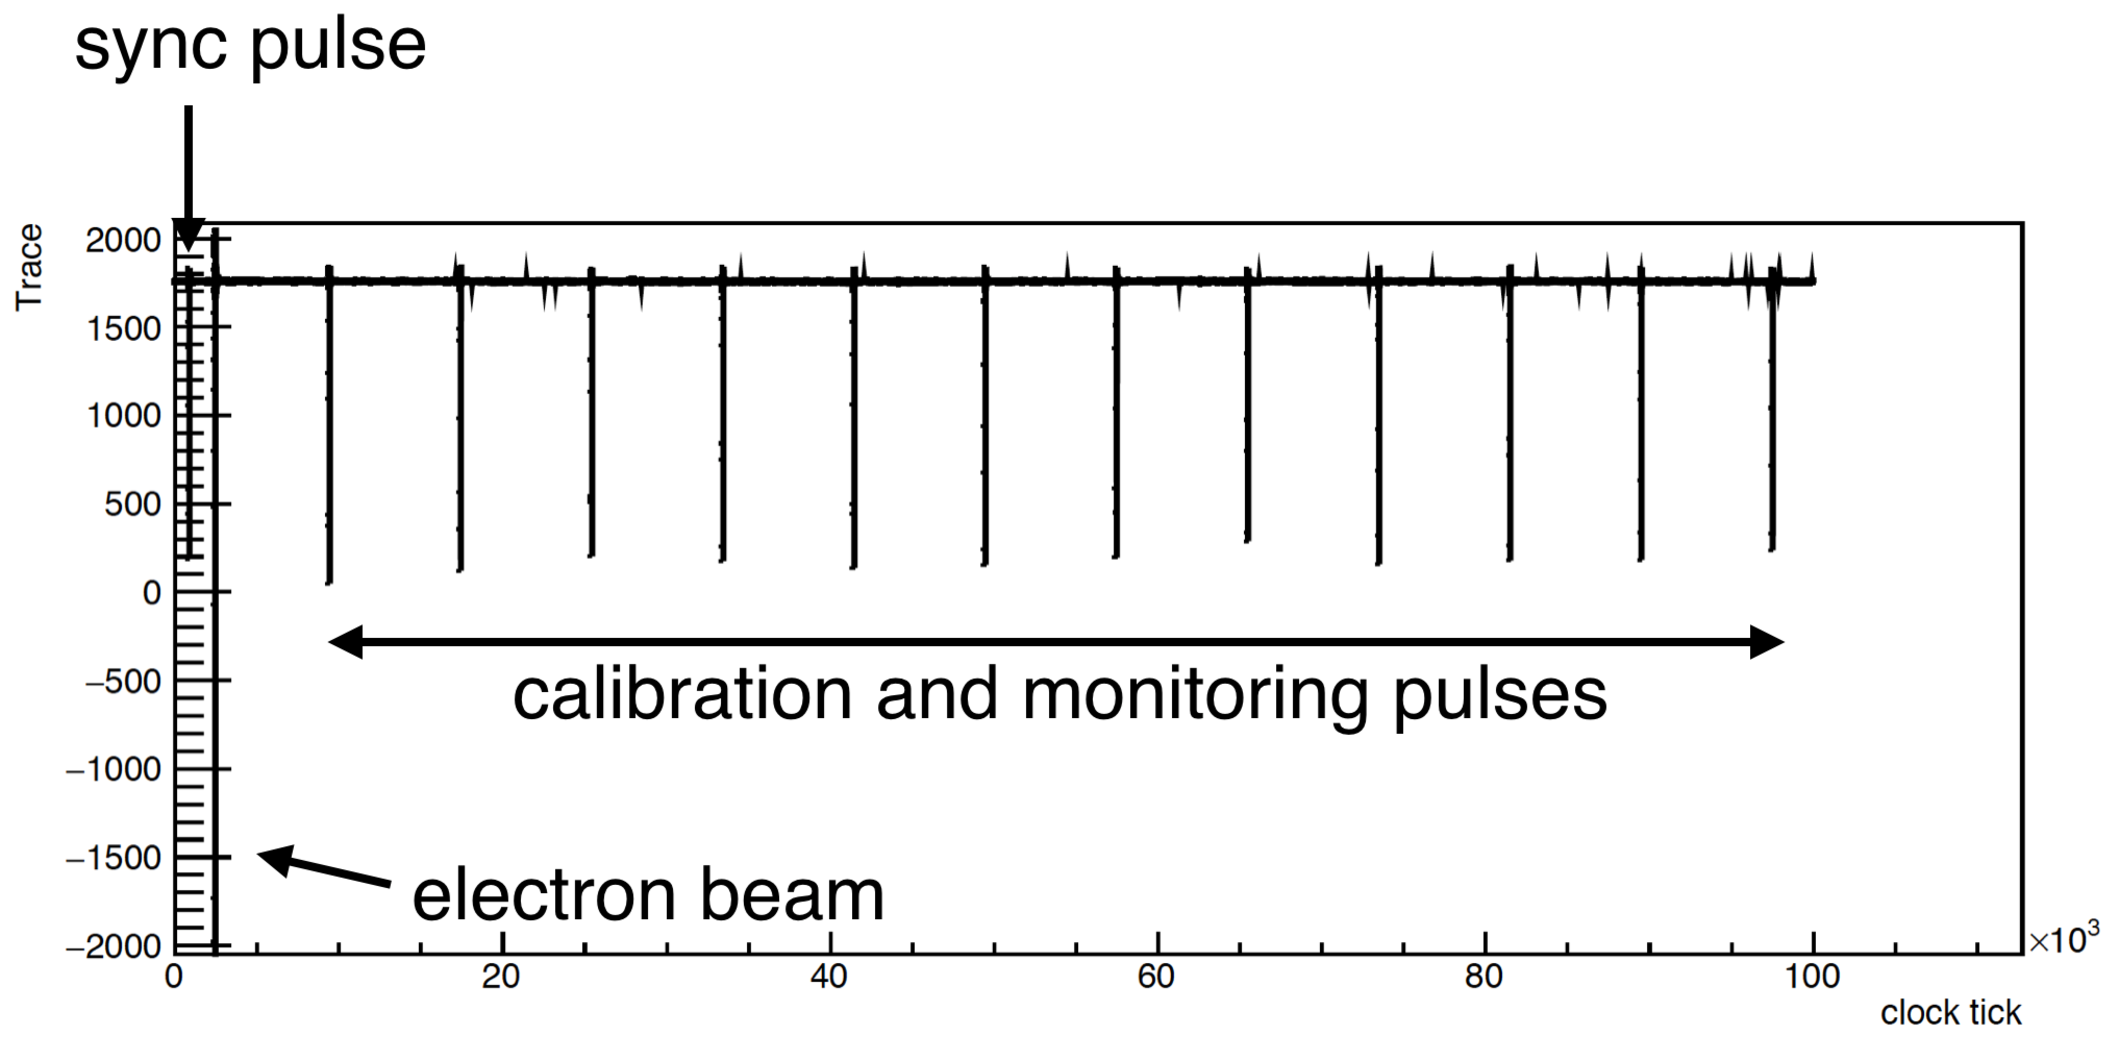
\includegraphics[width=.8\textwidth]{pics/eventtopology}
\caption{\label{fig:eventtopology} Event topology at SLAC.}
\end{figure}

\begin{table}[htbp]
\caption{Typical time and energy of sync, beam and laser pulses.}
\begin{longtable}{|c|c|c|c|} \hline
Pulse type & Time [c.t.] & Crystal hit E [p.e.] & Cluster E [p.e.] \\
\hline
Sync pulse	& $\approx$ 860, 0 (before, after corr.) &	1000-2000 &	60000-80000 \\
\hline
Beam pulse & $\approx$ 2500, $\approx$ 1600 (before, after corr.)	 & 0-2500 & 2500-3000 \\
\hline
Laser pulse	& $>$ 2860 c.t., $>$ 2000 c.t. (before, after corr.) & 1000-2000 & 60000-80000 \\
\hline
\end{longtable}
\end{table}

This chapter summarizes the program we have carried out during the SLAC run. For full program, please refer to \aref{app:program}.

\begin{itemize}
\item Vertical Sweep 
\item Calibration Sequnce
\item Template xtal 24 
\item Test PIX image of beam 
\item crystal centers in the cluster of 4x4 crystals
\item high statistics seg 24 
\item Fine position scan of segment 24 
\item Cross of 4 segments 
\item Edge scan outward of segment 26 
\item Crack scan 
\item Energy scan at 3 points for each 2.5, 3.5, 4.0, 4.5, 5.0 GeV 
\item Edge scan outward of segment 26 
\item Angle Scan at 5, 10, 15 and 25 degrees 
\item Moving Flight Simulator Tests
\item Fine vertical scan seg 24 
\item Horizontal scan seg 24 
\item Front face scan 
\item Undo wide islands for templates back to 8 pre-trigger, and 24 post-trigger 
\item Flight sim test, FW\#1, 96 shots per fill 
\item Low QE run 
\item Long run 
\item Horizontal scan of fiber harp 
\item Horizontal scan of fiber harp in calibration position, vertically centered in beam 
\item Scan of intensity and bias voltage 
\item Horizontal scan of fiber harp in calibration position with narrow beam 
\item Bias voltage scan 
\item Horizontal scan of fiber harp in calibration position, new beam width 
\item Scan of intensity and bias voltage at ideal position along fibers 
\item Long run at ideal position along fibers 
\item Long run with white paint on fiber ends 
\item Horizontal scan of fiber harp in calibration position with white paint 
\item Vertical scan of T0 counter 
\item Laser before beam at different time separations 
\end{itemize}
